%%%%%%%%%%%%%%%%%%%%%%%%%%%%%%%%%%%%%%%%%%

\chapter{LANL nEDM experiment control and data acquisition systems}\label{chap:daq}

%%%%%%%%%%%%%%%%%%%%%%%%%%%%%%%%%%%%%%%%%%

This chapter primarily serves as documentation regarding the experimental control system and data acquisition (\acrshort*{daq}) system for the LANL nEDM experiment. We first describe the devices associated with $\pi/2$ pulse generation in the Ramsey method (Secs.~\ref{sec:pulse_gen_freq_std}). We then describe the analog to digital conversion (\acrshort*{adc}) system responsible for recording the pulse height spectra and timing of UCN detection events (Sec.~\ref{sec:fast_daq}). Lastly, we describe the current iteration of the experimental control system (Sec.~\ref{sec:slow_control}) and the envisioned final version (Sec.~\ref{sec:web_control}).

The majority of the code implemented this chapter is extremely lengthy. In lieu of an appendix, we provide addresses to the repositories hosted on GitHub in the table below.

\begin{table}[htp]
\renewcommand*{\arraystretch}{2}
\centering
\caption{Links to code repositories}\label{tb:github}
\begin{tabular}{
    l
    r
}
\toprule
Description & \href{https://github.com/dougUCN/}{github.com/dougUCN} \\
\midrule
SIS3316 Digitizer  & \href{https://github.com/dougUCN/SIS3316}{/SIS3316} \\
\makecell[l]{GPIB device communication\\(DS345, DG535, BNC577)} & \href{https://github.com/dougUCN/gpibUSB}{/gpibUSB} \\
Cell valve motor control & \href{https://github.com/dougUCN/STM23Q}{/STM23Q} \\
Switcher motor control &  \href{https://github.com/dougUCN/H54-200-S500-R}{/H54-200-S500-R} \\
ZeroMQ Communication & \href{https://github.com/dougUCN/zmqLANL}{/zmqLANL} \\
SIS3316 GUI & \href{https://github.com/dougUCN/sis3316_gui}{/sis3316\_gui} \\
Web-based control system (FE) & \href{https://github.com/dougUCN/LANE-client}{/LANE-client} \\
Web-based control system (BE) & \href{https://github.com/dougUCN/LANE-server}{/LANE-server} \\
\bottomrule
\end{tabular}
\end{table}


%%%%%%%%%%%%%%%%%%%%%%%%%%%%%%%%%%%%%%%%%%

\section{RF signal generators and frequency standard}\label{sec:pulse_gen_freq_std}

%%%%%%%%%%%%%%%%%%%%%%%%%%%%%%%%%%%%%%%%%%

The frequency generators for the $\pi/2$ RF coils and other timing systems in the experiment must have smaller uncertainty than the counting statistics from a single measurement cycle. From Sec.~\ref{sec:lanl_nedm_uncertainty}, the nEDM uncertainty per Ramsey sequence measurement for two cells is on the order of $\sim 10^{-25}\,e\text{ cm}$. From Eq.~(\ref{eq:delta_omega_dipole_relation}), for $E=\qty{12}{kV\per cm}$ this gives a frequency uncertainty of $\sigma(f)\sim \qty{1}{\micro Hz}$.

We use SRS DS345 signal generators to drive the $\pi/2$ RF coils. The accuracy of the signal generators is stated to be \qty{5}{ppm}~\cite{ds345_manual}, which for the $\approx\qty{30}{Hz}$ resonance in the LANL nEDM Ramsey sequence (Sec.~\ref{sec:LANL_nEDM_ramsey_params}) corresponds to $\qty{0.15}{mHz}$. This can be improved to at least $\qty{0.1}{\micro Hz}$ per measurement with synchronization to a SRS FS725 rubidium frequency standard, which we have procured. The FS725 has short-term \qty{1}{s} stability (Allan variance) and accuracy to a few parts in $10^{11}$, and long-term \qty{20}{yr} accuracy of \num{5e-9}~\cite{rubidium_standard_fs725_manual}.

A frequency uncertainty specification of $\sim \qty{1}{\micro Hz}$ gives a phase shift uncertainty per Ramsey measurement of $\sigma(\phi)=2\pi\gls{T_fp}\,\sigma(f)\sim \qty{1}{mrad}$. We performed a phase stability test, where a $V_\text{S}=\qty{1}{V}$, $f_\text{S}=\qty{30}{Hz}$ signal from a DS345 was input into a Signal Recovery 7265 lock-in amplifier. A second $V_\text{R}=\qty{1}{V}$, $f_\text{R}=\qty{30}{Hz}$ signal from another DS345, referenced to the FS725, was the reference. The lock in time constant was \qty{200}{ms}. The output phase was $\Phi=2\pi \Delta f\,t-\Delta\phi(t)$ where $\Delta f=f_\text{R}-f_\text{S}$ and $\Delta\phi(t)$ is the phase drift of the signal DS345 relative to the FS725 standard. The output phase increased at a rate of $d\Phi/dt=\qty{1.16e-4}{rad\per s}$, which assuming $\Delta f$ is the dominant contribution implies $\Delta f=\qty{18}{\micro Hz}$ (a true frequency of $f_\text{S}=\qty{29.999982}{Hz}$) and an accuracy of $\qty{18}{\micro Hz}/\qty{30}{Hz}=\qty{0.6}{ppm}$. Setting the input signal frequency to $\qty{30.000018}{Hz}$ resulted in $d\Phi/dt=\qty{5.82}{\micro rad\per s}$, which sets a bound $d\phi(t)/dt<\qty{5.82}{\micro Hz\per s}$. Over the a $\gls*{T_fp}=\qty{180}{s}$ free precession this gives a maximum shift of $\qty{1.05}{mrad}$, matching the phase uncertainty specification for a DS345 that is unsynchronized to the FS725. We anticipate that the DS345 phase drift when synchronized to the time standard is significantly smaller.

%%%%%%%%%%%%%%%%%%%%%%%%%%%%%%%%%%%%%%%%%%

\subsection{RF pulse and free precession timing}\label{sec:pulse_gates}

%%%%%%%%%%%%%%%%%%%%%%%%%%%%%%%%%%%%%%%%%%

Timing of the $\pi/2$ pulses and free precession period has previously been controlled with a DG535 pulse generator (see measurements in Chap.~\ref{chap:lanl_ramsey_demonstration}). The DG535 was used to modulate the output amplitude of the DS345 function generator. The DG535 has a delay resolution of \qty{5}{ps}, and a nominal channel-to-channel jitter of \qty{50}{ps}~\cite{dg535_manual}. An 8-channel BNC577 pulse generator has also been procured in anticipation of additional instrumentation with precise timing requirements. The BNC577 has a delay resolution of \qty{250}{ps} and channel-to-channel jitter of \qty{50}{ps}~\cite{bnc_577_manual}. Both pulse generators may be synchronized to the FS725 time standard, which would further improve their performance.

%%%%%%%%%%%%%%%%%%%%%%%%%%%%%%%%%%%%%%%%%%

\section{Data acquisition}\label{sec:fast_daq}

%%%%%%%%%%%%%%%%%%%%%%%%%%%%%%%%%%%%%%%%%%

The ADC system has been rigorously tested, having been utilized in all nEDM commissioning measurements involving UCN detection since 2020. The signal conditioning chain after the detector is relatively minimal, and is described in Sec.~\ref{sec:signal_conditioning}. The LANL nEDM uses a \qty{250}{MHz} SIS3316 by Struck Innovative Systeme to digitize the conditioned output. A RESTful interface was originally written by Sergey Ryzhikov for the PANDA experiment at the Institute for High Energy Physics, but it was written in Python2 and had lost compatibility with any SIS3316 with firmware later than 2015. An updated version in Python3, compatible with all firmware released to date and with an expanded feature set, is at the repository listed in Tab.~\ref{tb:github}. 

The manuals for the SIS3316~\cite{sis3316_manual, sis3316_udp_addendum} (available on the GitHub repository) provide ample documentation, but we highlight relevant specifications, triggering algorithms, and device communication protocols in Sec.~\ref{sec:sis3316_specs}--\ref{sec:sis3316_data_format}.

%%%%%%%%%%%%%%%%%%%%%%%%%%%%%%%%%%%%%%%%%%

\subsection{UCN detection signal conditioning}\label{sec:signal_conditioning}

%%%%%%%%%%%%%%%%%%%%%%%%%%%%%%%%%%%%%%%%%%

 \begin{figure}
    \centering
    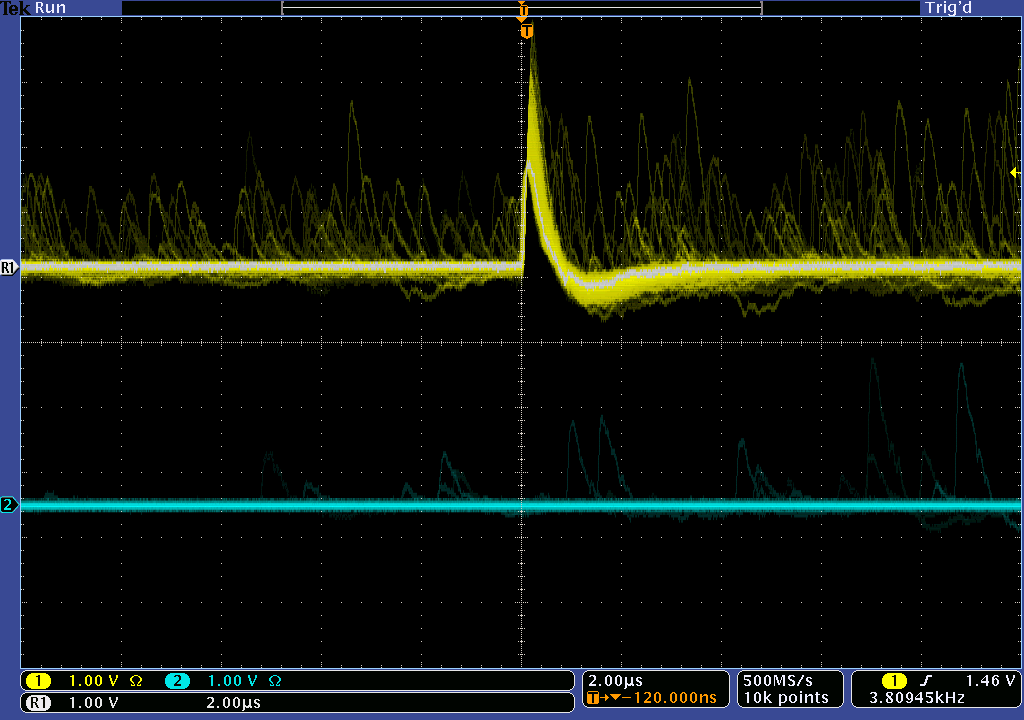
\includegraphics[width=0.8\textwidth]{figures/pmt_scope.png}
    \caption
     {UCN signals as viewed on an oscilloscope, after the PMT output is processed by an Ortec 474 timing filter amplifier}
    \label{fig:scope_image}
\end{figure}

After UCN are detected as per Sec.~\ref{sec:ucn_detectors}, the signal output from a \gls*{pmt} is sent to an Ortec 474 timing filter amplifier. The integration time is set to \qty{500}{\nano\second}. Gain is set such that the pulse spectrum heights, when viewed on an oscilloscope, have an amplitude $\sim\qty{1}{\volt}$. The differentiation time is nominally in the range of 0--\qty{20}{\nano\second}, set such that the pulse decays within \qty{5}{\micro \second}. An example UCN pulse shape as viewed on an oscilloscope after signal conditioning is shown in Fig.~\ref{fig:scope_image}.

Initial tests of UCN with Onsemi \acrshort*{sipm} 4-Side Scaleable Arrays (C Series), used on the simultaneous spin analyzers (Chap.~\ref{chap:ssa_2020}), have shown that \acrshort*{sipm} the output only needs a multiplicative gain for improved peak height sprectra resolution, and does not require the same pulse shaping as the PMTs. A custom fast-amplifier is being designed and built.

%%%%%%%%%%%%%%%%%%%%%%%%%%%%%%%%%%%%%%%%%%

\subsection{Struck SIS3316 specifications}\label{sec:sis3316_specs}

%%%%%%%%%%%%%%%%%%%%%%%%%%%%%%%%%%%%%%%%%%

The SIS3316 used in the LANL nEDM for ADC is the 16-channel SIS3316-250-14, which has a \qty{250}{MHz} sampling rate with 14-bit pulse height resolution. It supports using either an internal clock oscillator (Silicon Labs SI570) or an external \qty{10}{MHz} clock input in combination with a programmable clock multiplier.

The SIS3316 supports complete logging of the ADC waveform, though this is not recommended due to exorbitant file size. As an alternative, the user may define up to 8 ``accumulation periods,'' where after a trigger, the SIS3316 provides an integrated sum over the waveform for the defined periods.

Dead time, when the SIS3316 is unable to act after an event trigger, is typically on the order of $\sim\qty{100}{ns}$ for nominal configurations. If the SIS3316 has been instructed to log the entire waveform the dead time approaches $\sim\qty{1}{\micro s}$.


%%%%%%%%%%%%%%%%%%%%%%%%%%%%%%%%%%%%%%%%%%

\subsection{Communication with the SIS3316}\label{sec:sis3316_udp_protocol}

%%%%%%%%%%%%%%%%%%%%%%%%%%%%%%%%%%%%%%%%%%

In this section we provide an introduction to the user datagram protocol (UDP) for communication with the SIS3316. We refer to the initiator of the command as the ``client'' and the recipient (the SIS3316) as the ``server.''

VME FPGA refers to a system that uses Versa Module Europa (VME) as the bus standard for interconnecting modules and Field Programmable Gate Arrays (FPGA) for implementing custom logic. The SIS3316 VME FPGA communication protocol is as depicted in Fig.~\ref{fig:sis3316_read_write_ack}. It is primarily used for reading and writing settings to the ADC. The client sends a command, consisting of a header (0x10 for a read request, 0x11 for a write command) to the SIS3316. The client's command contains an arbitrary packet identifier, which can be used for client-side validation when the server acknowledges the command in a read request reply. The client command also contains an address. For a read request, this elicits a response from the SIS3316, where the returned data is from the specified address. A write command from the client includes both an address and the data to write to the address, which receives no acknowledgement from the server.

\begin{figure}
    \centering
    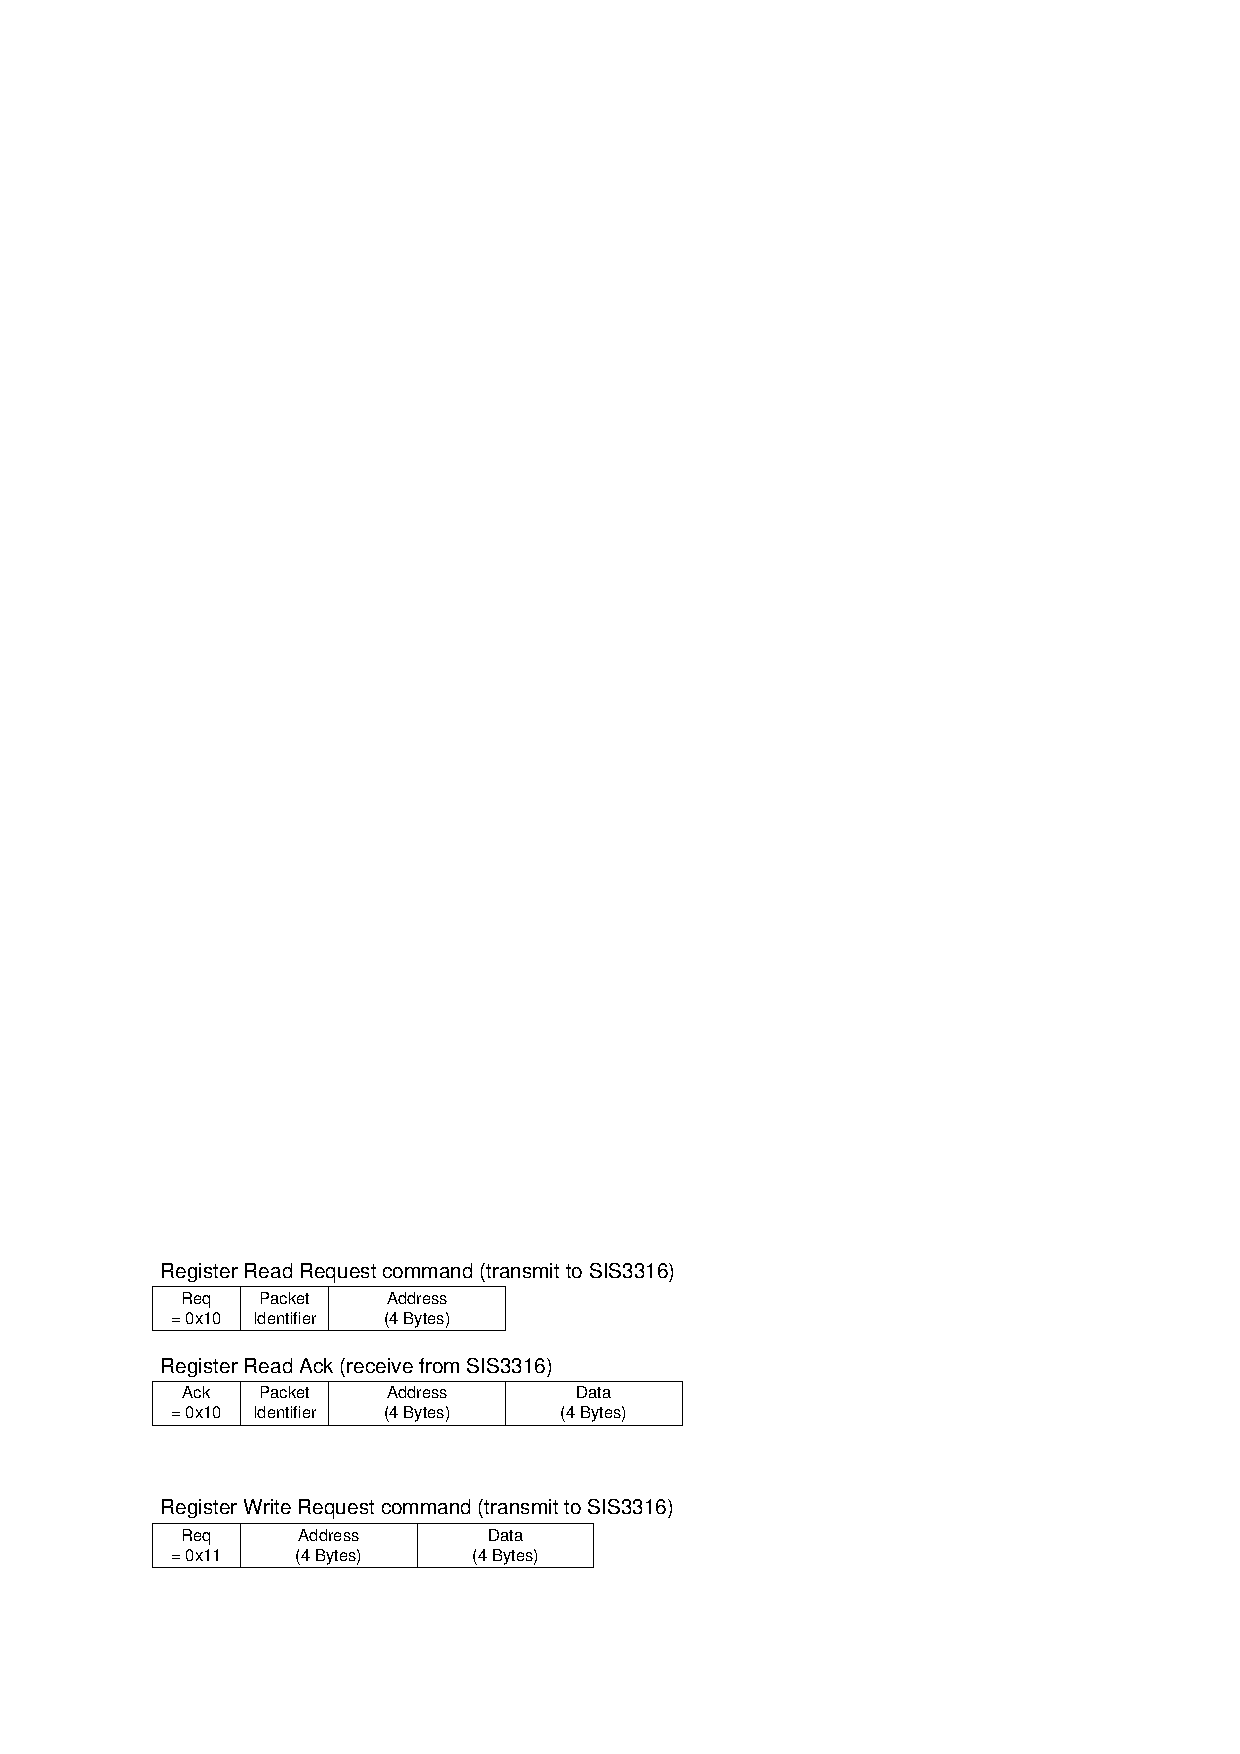
\includegraphics[height=2in]{figures/sis3316_ethernet_ack.pdf}
    \caption
    [VME FPGA Access protocol for the SIS3316.]
     {VME FPGA Access protocol for the SIS3316. Page 12 of Ref.~\cite{sis3316_udp_addendum}}
    \label{fig:sis3316_read_write_ack}
\end{figure}

The first in first out (FIFO) space readout communication protocol is depicted in Fig.~\ref{fig:sis3316_fifo}. It is primarily used to stream ADC data of detected UCN from the server to the client.

\begin{figure}
    \centering
    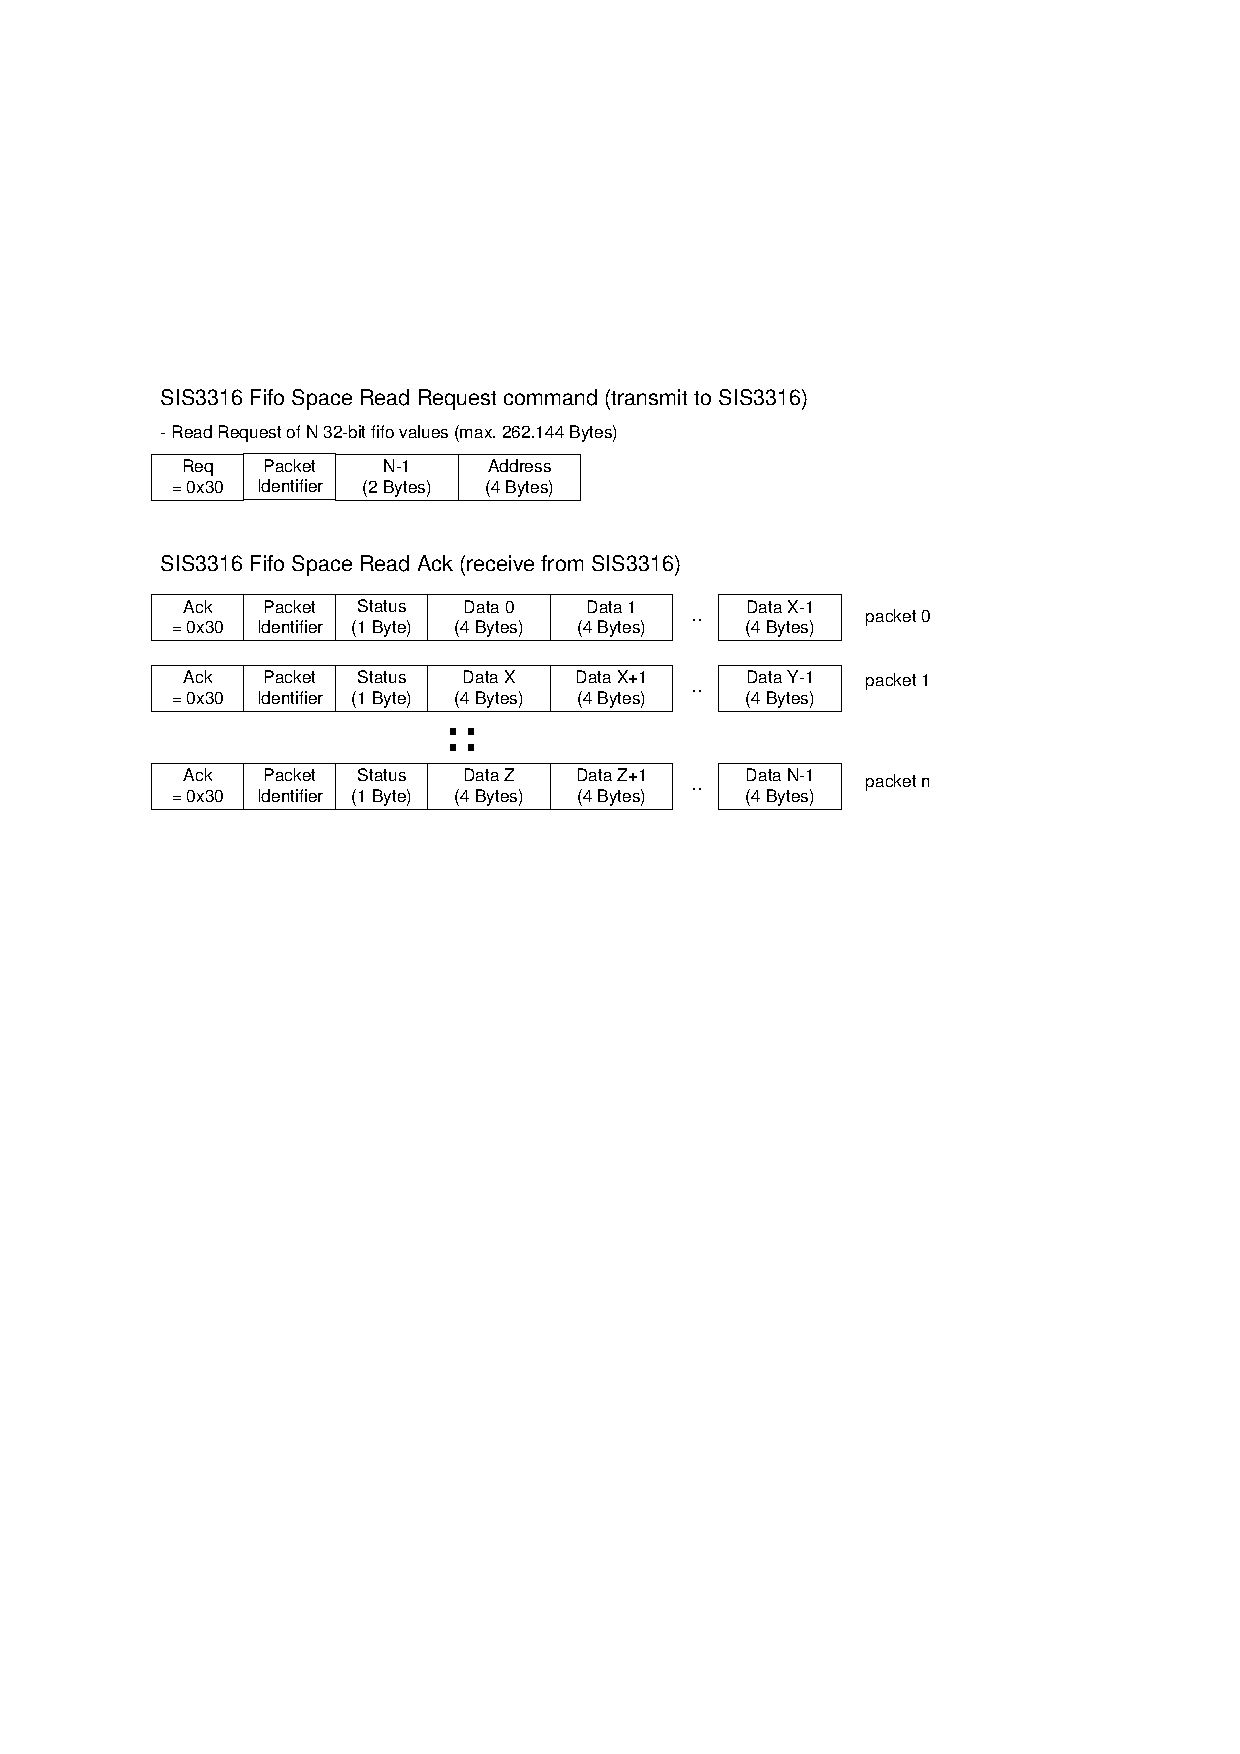
\includegraphics[height=2.5in]{figures/sis3316_fifo.pdf}
    \caption
    [SIS3316 Fifo space read request and acknowledgement.]
     {SIS3316 Fifo space read request and acknowledgement. Page 17 of Ref.~\cite{sis3316_udp_addendum}}
    \label{fig:sis3316_fifo}
\end{figure}


The LANL nEDM fast DAQ uses an Ethernet interface with the SIS3316. Configuration instructions with regards to IP address assignment is located in the code repository. Ethernet offers the benefit of a very large bandwidth. In order to maximize the data transfer rate, reduce the total number of packets sent, and reduce the chances of a packet being dropped, we direct the SIS3316 to use Jumbo frames, with a maximum transmission unit (MTU) of 9000 bytes. This essentially maximizes the per-envelope data transfer.


%%%%%%%%%%%%%%%%%%%%%%%%%%%%%%%%%%%%%%%%%%

\subsection{Trapezoid trigger algorithm}

%%%%%%%%%%%%%%%%%%%%%%%%%%%%%%%%%%%%%%%%%%

The algorithm for the SIS3316 that determines whether or not an event should be logged is called a ``trapezoid trigger,'' which uses two running averages of the same ADC signal. Two parameters, peaking and gap time, affect the shape of the trapezoid.

As depicted in Fig.~\ref{fig:sis3316_trapezoid}, a moving average window, determined by peaking time, is applied to an ADC signal. Some gap time later, a second moving average of the same ADC signal is created. The difference of the two moving averages creates the trapezoid.


\begin{figure}
    \centering
    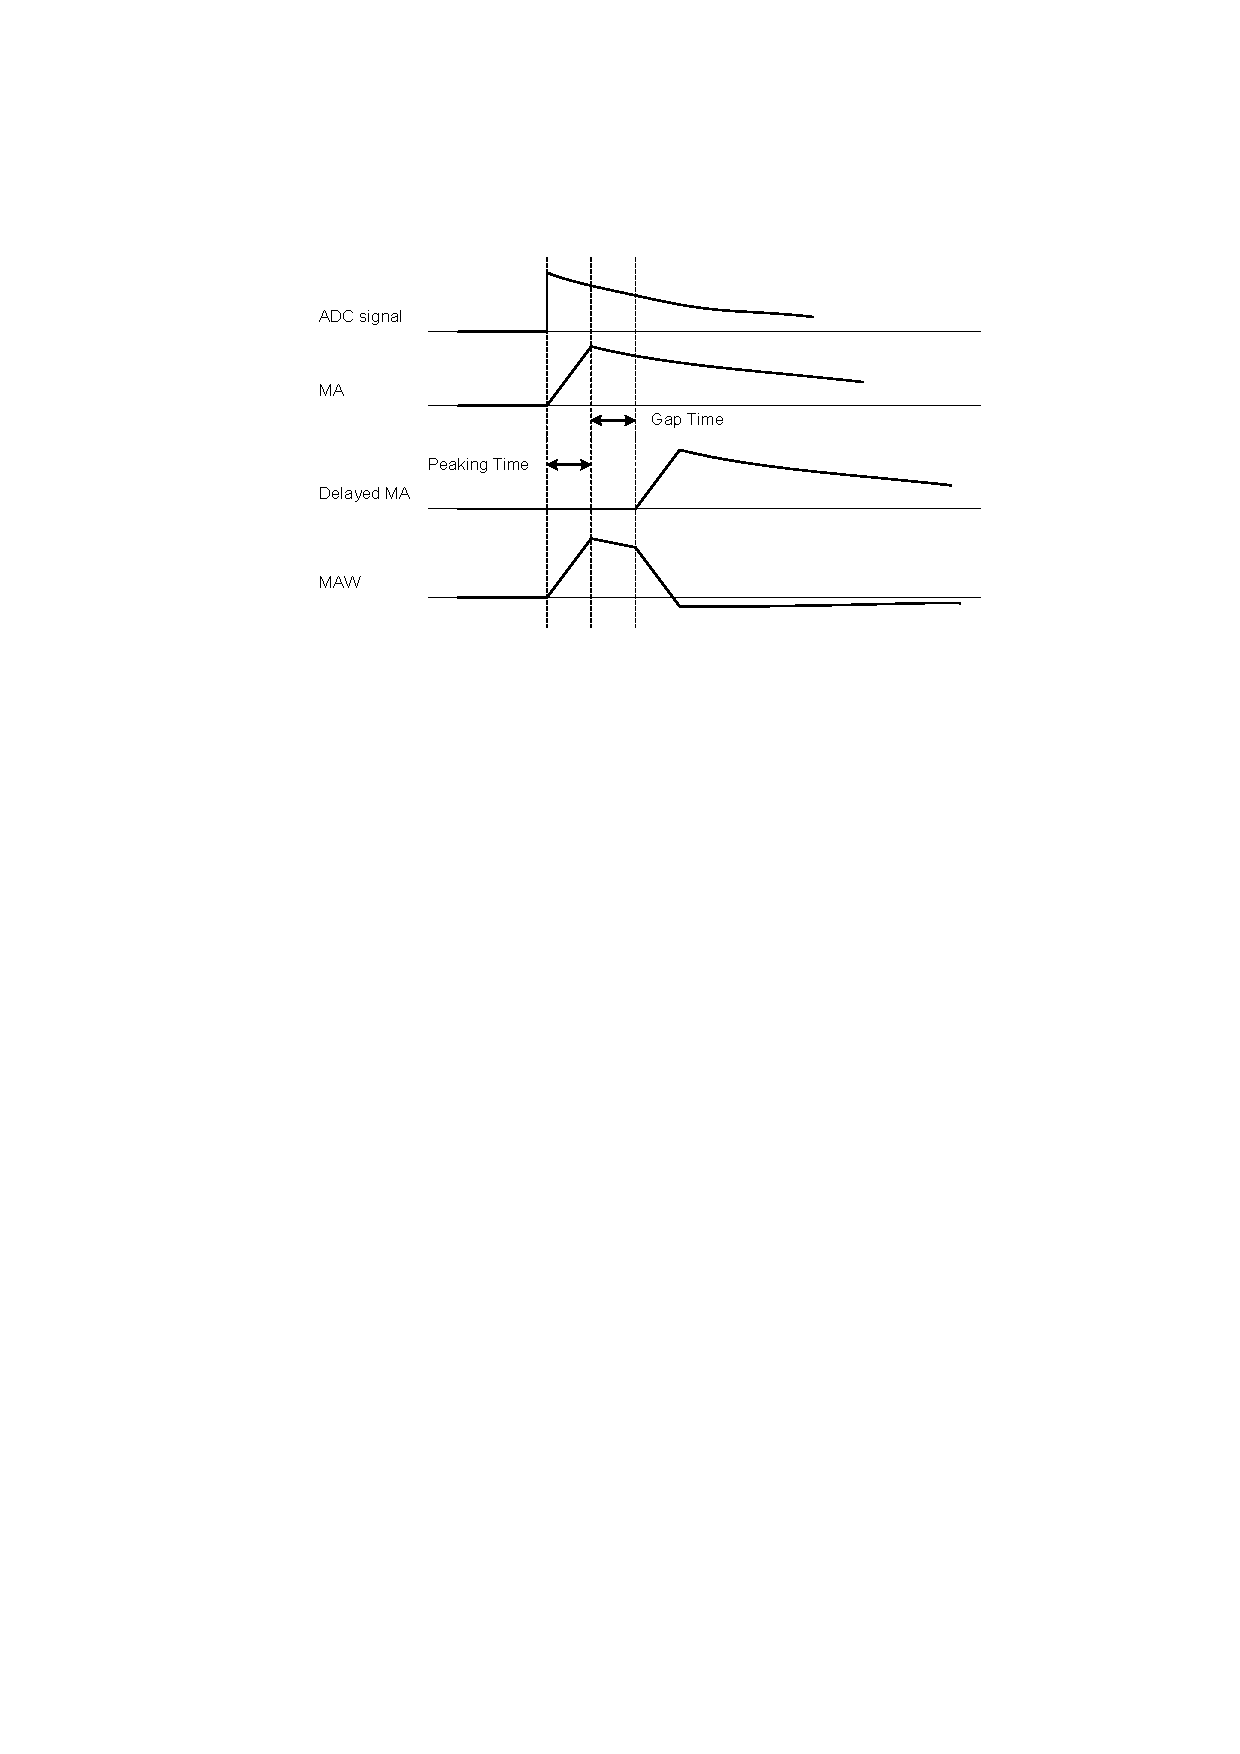
\includegraphics[height=2.5in]{figures/sis3316_trapezoid.pdf}
    \caption
    [Trapezoid trigger algorithm of the SIS3316.]
     {Trapezoid trigger algorithm of the SIS3316. Page 50 of Ref.~\cite{sis3316_manual}}
    \label{fig:sis3316_trapezoid}
\end{figure}

The trigger is armed when the trapezoid is above the user-defined trigger threshold, and counts the event when the trapezoid drops below 50\% of its maximum height. The trigger can be changed to simply trigger when the trapezoid is above some threshold.

A pileup event occurs if a second ADC event occurs during the same trigger gate window as an already triggered event. The trapezoid algorithm is uniquely equipped to identify such events, as seen in pages 66--67 of Ref.~\cite{sis3316_manual}. A pileup signal manifests as a binary flag in the output data, per Fig.~\ref{fig:sis3316_raw_data}. A repileup option is also available, which allows triggering on the second ADC event.


%%%%%%%%%%%%%%%%%%%%%%%%%%%%%%%%%%%%%%%%%%

\subsection{Data format}\label{sec:sis3316_data_format}

%%%%%%%%%%%%%%%%%%%%%%%%%%%%%%%%%%%%%%%%%%

The binary data output format streamed from the SIS3316 to the client is as indicated in Fig.~\ref{fig:sis3316_raw_data}. The configuration of the header changes depending on the format setting instruction applied to the SIS3316 (optional fields colored green, yelow, orange, and blue). After a completed run, the LANL nEDM experiment rewrites the data to HDF5. For production data, a blinding factor will be applied during this rewriting, or ``replay,'' phase. 


\begin{figure}
    \centering
    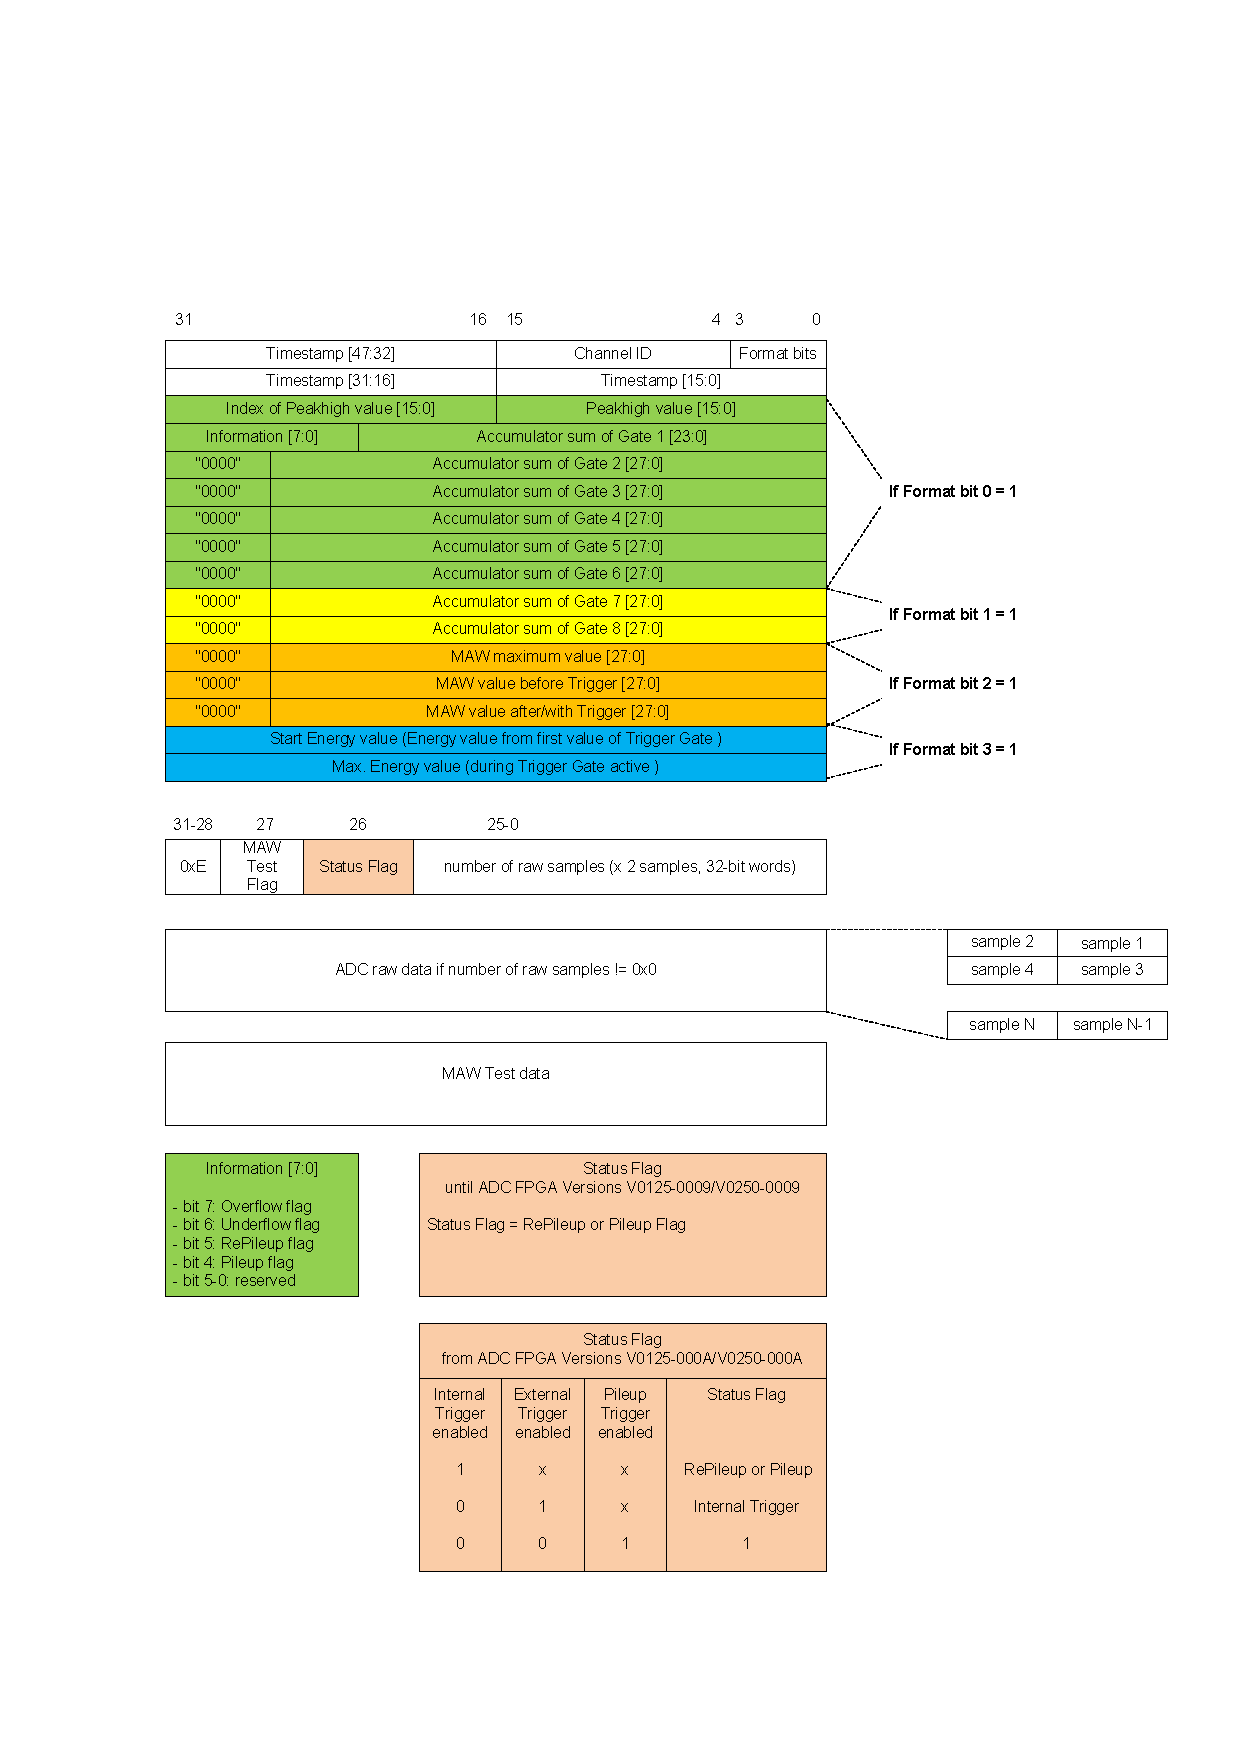
\includegraphics[height=0.9\textheight]{figures/sis3316_raw_data.pdf}
    \caption
    [Binary data output format of an ADC event for the SIS3316.]
     {Binary data output format of an ADC event for the SIS3316. Page 69 of Ref.~\cite{sis3316_manual}}
    \label{fig:sis3316_raw_data}
\end{figure}

%%%%%%%%%%%%%%%%%%%%%%%%%%%%%%%%%%%%%%%%%%

\subsection{Data blinding}\label{sec:sis3316_data_blinding}

%%%%%%%%%%%%%%%%%%%%%%%%%%%%%%%%%%%%%%%%%%

We conclude the overview of the ADC system with a brief discussion regarding the data blinding procedure and its close ties to ADC performance. Data blinding is an important procedure that occurs during collection of production data, designed to remove psychological bias during the analysis. For nEDM experiments, one such procedure has been to shift the minimum of the Ramsey fringe with a fake nEDM signal, as in Ref.~\cite{Ayres_psi_data_blinding_2021}. This is accomplished with a small, coordinated shift in the number of counted UCN in the quadruplet of runs along the central peak ($\omega_1$--$\omega_4$ in Fig.~\ref{fig:ramsey-sequence}). For a blinded nEDM shift of $\num{1e-25}\,e\text{ cm}$, this results in an alteration of $\approx 3$ UCN counts per run~\cite{Ayres_psi_data_blinding_2021}.

Special care must be taken towards pileup events, which can easily asymmetrically alter counts per individual run (as opposed to, for example, trigger thresholds, which would affect all runs in the quadruplet equally). For the SIS3316, the accumulator gates, pileup, and repileup settings can be used to provide insight into pileup events, but will need to be further refined in coming UCN measurement cycles. Other blinding options that do not involve UCN count shifts of the same magnitude as pileup uncertainty should also be explored.

%%%%%%%%%%%%%%%%%%%%%%%%%%%%%%%%%%%%%%%%%%

\section{Experiment control}\label{sec:slow_control}

%%%%%%%%%%%%%%%%%%%%%%%%%%%%%%%%%%%%%%%%%%

This section describes the ``slow control,'' in reference to systems in the experiment that are not particularly high-bandwidth. A LabJack-U3-LV with a PS12DC Power Switching Board attachment is used to communicate with the proton accelerator, beamline gate valves, and other systems that require a transistor-transistor logic (TTL) pulse for control. The UCN switchers (Sec.~\ref{sec:lanl_switchers}) are actuated by Dynamixel H54-200-S500-R motors, controlled via USB serial interface. The UCN cell valves are actuated by STM23Q motors from Applied Motion Products over a direct Ethernet interface, with a Netgear GS308 Switcher used to support the control of multiple motors with limited ethernet ports. A general user interface (GUI) written using PyQt sends start/stop signals to the SIS3316, supports loading of configuration files into the SIS3316, and provides live histograms of pulse height spectra and UCN detector rate during measurements. 

For more timing-dependent devices, the slow control sends a series of commands to an intermediary BNC577 or DG535 pulse generator, to which the timing-dependent device is attached. The pulse generator programmed with the desired pulse sequence, and is set to externally trigger on a TTL pulse from the LabJack. The pulse generator then applies the programmed pulse sequence to the timing dependent device.

Code repositories and documentation for the SIS3316 GUI, UCN switcher control, GPIB device interfacing, and cell valve motor control are listed in Tab.~\ref{tb:github}.

%%%%%%%%%%%%%%%%%%%%%%%%%%%%%%%%%%%%%%%%%%

\subsection{ZeroMQ device network}

%%%%%%%%%%%%%%%%%%%%%%%%%%%%%%%%%%%%%%%%%%

For inter-thread communication on the same computer, or for inter-computer communications on the LANL network, we use ZeroMQ (ZMQ), an asychronous messaging library available for a broad body of languages. The use of this protocol allows collaborators from multiple universities to independently develop an experimental subsystem, as integration into the LANL experiment control system simply requires being compatible with ZMQ communications.

For the LANL nEDM control layout, we have multiple worker servers, such threads managing the ADC, magnetometer readouts, and other environmental monitoring services. The worker servers may or may not be located on the same computers. These workers are designated as ZMQ dealers. The worker servers wait for commands from the the main control system, designated as a ZMQ router. It is of note that the main control system sends commands without waiting for responses to avoid hanging if a worker server is inactive or unresponsive.

The worker servers, upon receiving commands, will perform tasks and send outbound response messages via a ZMQ push action. The responses are added to a ZMQ queue that is hosted on the main control system. The main control system can then check the queue messages via a ZMQ pull action at its leisure.

Code of a wrapper library that simplifies ZMQ configuration is provided in the repository listed in Tab.~\ref{tb:github}. In tests on the LANL network it has been shown that the robustness of the communication protocol will be greatly improved if the main control system issues redundant commands to the worker servers.

%%%%%%%%%%%%%%%%%%%%%%%%%%%%%%%%%%%%%%%%%%

\section{Web-based control system: proof of concept}\label{sec:web_control}

%%%%%%%%%%%%%%%%%%%%%%%%%%%%%%%%%%%%%%%%%%

\begin{figure}
    \centering
    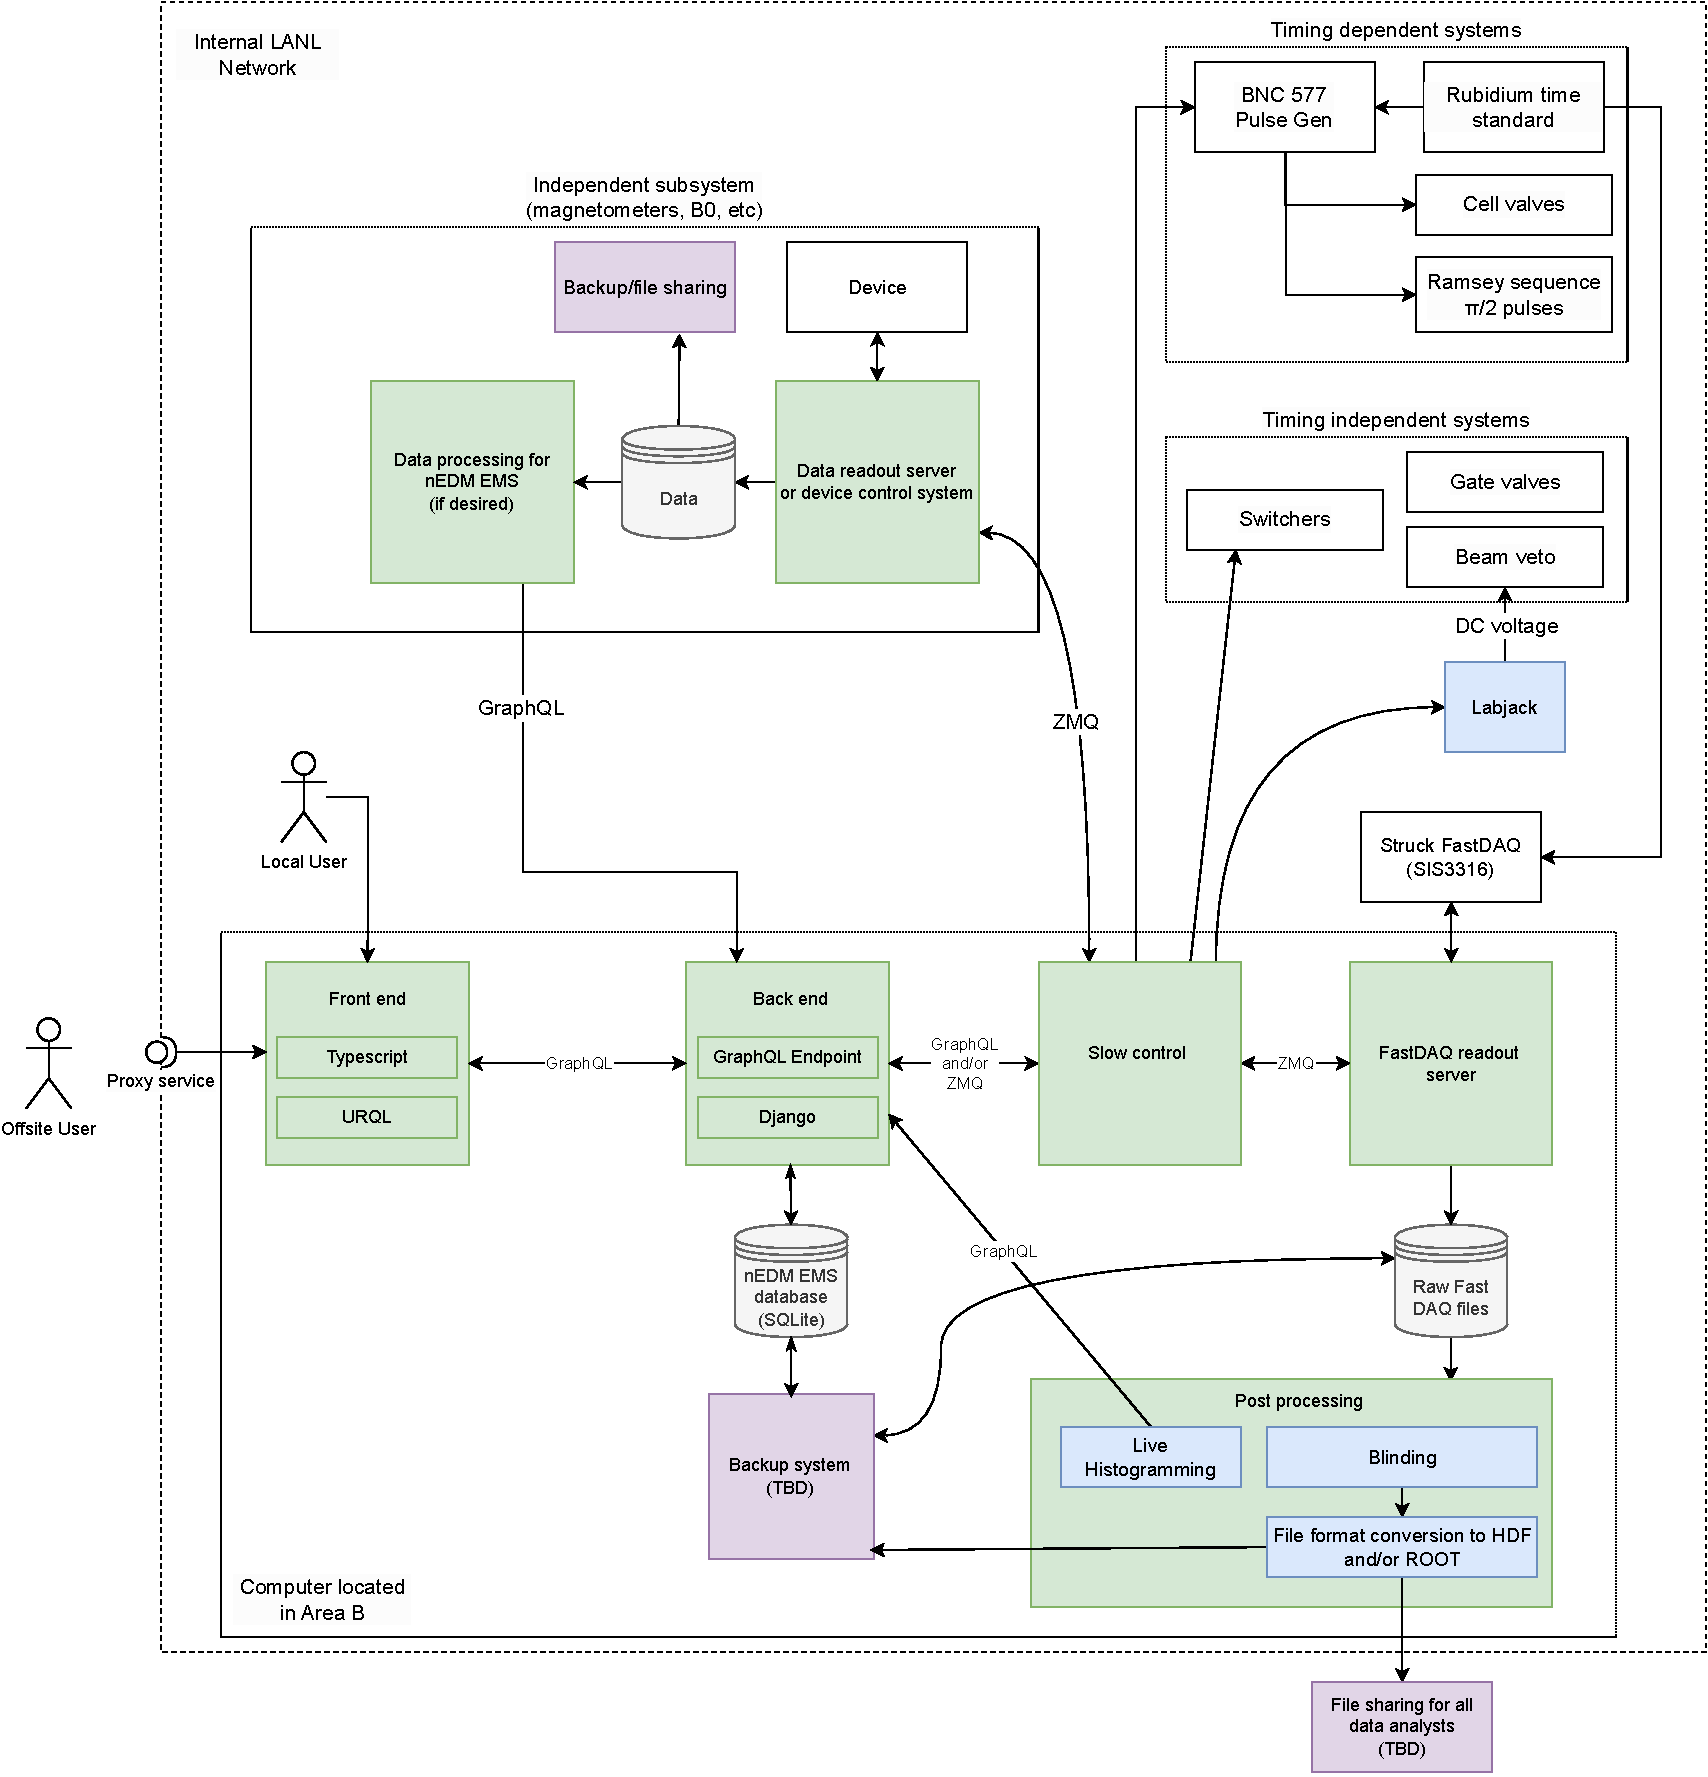
\includegraphics[width=\textwidth]{figures/LANL_nEDM_network.pdf}
    \caption
    [The eventual envisioned experiment control system at LANL]
     {The eventual envisioned experiment control system at LANL, as described in Sec.~\ref{sec:web_control} and demonstrated with a proof of concept. Each green box represents a computer thread. Code hosted at repositories listed in Tab.~\ref{tb:github}}
    \label{fig:LANL_nEDM_network}
\end{figure}

An upgraded, web-based version of the LANL nEDM experiment control is being developed, and a proof-of-concept has been completed. The web based version allows multiple users on the LANL internal network to access experiment control and environmental monitoring systems. Once issues with the LANL proxy web portal are resolved, off-site users will also be able to the view the experiment. The envisioned experiment control system network is depicted in Fig.~\ref{fig:LANL_nEDM_network}.

A front end server written in Typescript displays plots of past and current experimental measurements, and enables creation and editing of customized run configuration files that control the experiment. A back end server written in python Django interfaces with an SQLite database and forwards run configuration files to the slow control thread to run. The back end has an application programming interface (API) implemented using GraphQL. It offers several advantages over REST APIs: it is strongly typed, supports flexible querying, and is self-documenting with an introspection system. The front end server interacts with the back end using the URQL library to generate GraphQL posts.

When the slow control thread gets or fetches a run configuration from the back end, it sends out appropriate commands over ZMQ, LabJack, GPIB, and USB serial to the devices and threads involved in running the experiment. This includes communicating with pulse generator intermediaries for the timing dependent sequencing. Data collected by the SIS3316 ADC and other monitoring systems can be reported to the back end over GraphQL for display on the front end.

A proof-of-concept has been deployed on the internal LANL network, and is ready for testing in a measurement cycle. Nginx, a reverse proxy, is used to appropriately direct an incoming request to either the front end or back end server. Process managers ensure that the web service restarts upon crashes or server reboots. The front end server is monitored by the PM2 and the back end is monitored by Supervisor.

Additional documentation is located on the front end and back end code bases listed in Tab.~\ref{tb:github}.